\documentclass[a4paper, 12pt]{article}

\usepackage[utf8x]{inputenc}
\usepackage[T1]{fontenc}
\usepackage[francais]{babel}
\usepackage{xcolor}
\usepackage{listings}
\usepackage{mathptmx}
\usepackage{anyfontsize}
\usepackage{t1enc}
\usepackage[top=2cm, bottom=2cm, left=2cm, right=2cm]{geometry}
\usepackage{titlesec}
\usepackage{titling}
\usepackage{graphicx}
\usepackage{csquotes}
\usepackage{mdframed}
\definecolor{light-gray}{gray}{0.95}
\usepackage[colorlinks = true,
            linkcolor = black,
            urlcolor  = black,
            citecolor = black,
            anchorcolor = black]{hyperref}

\newcommand{\changeurlcolor}[1]{\hypersetup{urlcolor=#1}}

\renewcommand\maketitlehooka{\null\mbox{}\vfill}
\renewcommand\maketitlehookd{\vfill\null}

\definecolor{codegreen}{rgb}{0,0.6,0}
\definecolor{codegray}{rgb}{0.5,0.5,0.5}
\definecolor{codepurple}{rgb}{0.58,0,0.82}
\definecolor{backcolour}{rgb}{0.95,0.95,0.92}
\definecolor{codekeywords}{rgb}{0.1,0.53,0.92}

\lstdefinestyle{c++}{
    backgroundcolor=\color{backcolour},   
    commentstyle=\color{codegreen},
    keywordstyle=\color{codekeywords},
    numberstyle=\tiny\color{codegray},
    stringstyle=\color{codepurple},
    basicstyle=\ttfamily\footnotesize,
    breakatwhitespace=false,         
    breaklines=true,                 
    captionpos=b,                    
    keepspaces=true,                 
    numbers=left,                    
    numbersep=5pt,                  
    showspaces=false,                
    showstringspaces=false,
    showtabs=false,                  
    tabsize=2,
    texcl=false,
    inputencoding=utf8x,
    extendedchars=true,
    literate=
  {á}{{\'a}}1 {é}{{\'e}}1 {í}{{\'i}}1 {ó}{{\'o}}1 {ú}{{\'u}}1
  {Á}{{\'A}}1 {É}{{\'E}}1 {Í}{{\'I}}1 {Ó}{{\'O}}1 {Ú}{{\'U}}1
  {à}{{\`a}}1 {è}{{\`e}}1 {ì}{{\`i}}1 {ò}{{\`o}}1 {ù}{{\`u}}1
  {À}{{\`A}}1 {È}{{\'E}}1 {Ì}{{\`I}}1 {Ò}{{\`O}}1 {Ù}{{\`U}}1
  {ä}{{\"a}}1 {ë}{{\"e}}1 {ï}{{\"i}}1 {ö}{{\"o}}1 {ü}{{\"u}}1
  {Ä}{{\"A}}1 {Ë}{{\"E}}1 {Ï}{{\"I}}1 {Ö}{{\"O}}1 {Ü}{{\"U}}1
  {â}{{\^a}}1 {ê}{{\^e}}1 {î}{{\^i}}1 {ô}{{\^o}}1 {û}{{\^u}}1
  {Â}{{\^A}}1 {Ê}{{\^E}}1 {Î}{{\^I}}1 {Ô}{{\^O}}1 {Û}{{\^U}}1
  {œ}{{\oe}}1 {Œ}{{\OE}}1 {æ}{{\ae}}1 {Æ}{{\AE}}1 {ß}{{\ss}}1
  {ç}{{\c c}}1 {Ç}{{\c C}}1 {ø}{{\o}}1 {å}{{\r a}}1 {Å}{{\r A}}1
  {€}{{\EUR}}1 {£}{{\pounds}}1
  {├}{|}1 {─}{--}1 {└}{+}1
}
\lstset{style=c++}


\title{Simulation TP5\\Architecture Logicielle et Qualité\\Système Multi-Agents}
\author{Arquillière Mathieu - Zangla Jérémy}
\date{\today}


\begin{document}

\begin{titlepage}
  \maketitle
\end{titlepage}

\tableofcontents
\listoffigures
\newpage


% =========================================================== %
%                        Introduction
% =========================================================== %

\section{Introduction}
Ce document fait suite aux \changeurlcolor{blue}\href{run:../CahierDesCharges/cahier.pdf}{cahier des charges} concernant
un système multi-agents. Il s'agit donc de réaliser un système avec les agents décrit dans ce cahier des charges.
Pour cela on utilisera le langage C++, avec la librairie standard fournie avec. Pour la compilation, on utilisera g++
avec un makefile et enfin Doxygen pour la documentation associée à ce projet.


% =========================================================== %
%                        Organisation
% =========================================================== %

\section{Organisation}
\subsection{Arborescence}
\begin{figure}[!h]
  \centering
  \caption{Résultat de la commande \emph{tree}}
  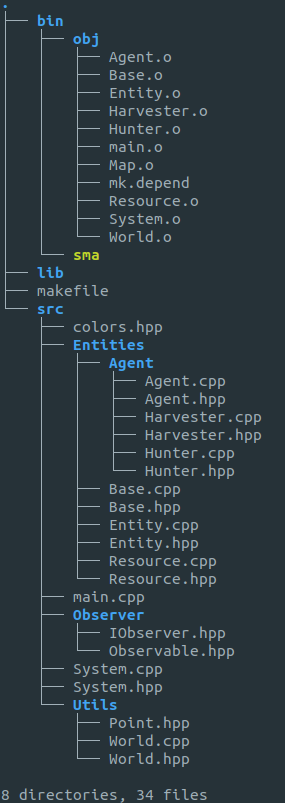
\includegraphics[scale=0.5]{img/tree.png}
\end{figure}

\subsection{Fonctionnement}
Nous avons vu précédemment dans le cahier des charges le comportement de chaque agent et les relations entre les objets.
Ici nous allons nous intéresser au fonctionnement globale qui est un peu différent de ce que nous avions prévu. Par exemple,
la classe \emph{System} était censée être à la fois la classe qui "s"occupe" des agents mais aussi représenter leur
monde, leur environnement. Cependant nous nous sommes rendu compte après avoir essayé de cette façon que cela compliquait
les choses puisque les agents doivent pouvoir obtenir des informations sur leur environnement et le modifier (via le système) et que
celui-ci s'occupe de les animer. Cette relation à double sens était trop compliquer à gérer et nous avons décidé de scinder
la classe \emph{System} en deux, d'une part le vrai système, qui s'occupe des agents et d'autre part le "monde", l'environnement
2D dans lequel évoluent les agents. Cela nous a permis de bien séparer les fonctionnalités.
On a désormais la classe \emph{World} qui gère les déplacements de chaque agent et peut leur fournir
des informations sur leur environnement.

\subsection{Patrons de conception}
\subsubsection{Observer}
Afin de gérer la séparation des tâches entre la classe \emph{System} et la classe \emph{World},
on a mis en place un patron \emph{Observer}.
\begin{figure}[!h]
  \centering
  \caption{Diagramme de classe du patron \emph{Observer} (source: \href{http://www.goprod.bouhours.net/?page=pattern&pat_id=16}{Site de M.Bouhours})}
  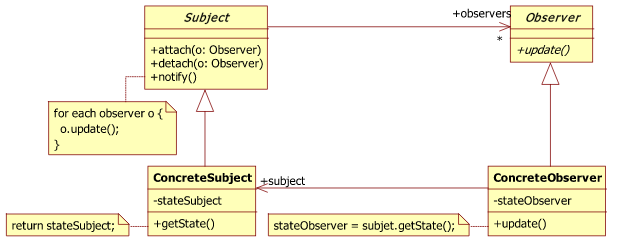
\includegraphics[scale=0.7]{img/observer.png}
\end{figure}

Dans notre cas, les \emph{Observable} sont les agents et les \emph{Observer} sont le système et le world.
L'implémentation de ces 2 classes se fait de la manière suivante :
\begin{figure}[!h]
  \centering
  \caption{Interface \emph{Observer}}
  \lstinputlisting[language=c++, firstline=21, lastline=43]{../Code/src/Observer/IObserver.hpp}
\end{figure}

\begin{figure}[!h]
  \centering
  \caption{Classe \emph{Observable}}
  \lstinputlisting[language=c++, firstline=23, lastline=65]{../Code/src/Observer/Observable.hpp}
\end{figure}

Ce patron permet aux classes \emph{System} et \emph{World} de faire une action en conséquence d'un déplacement
ou d'une mort d'une entité provoquée par un agent. Par exemple le \emph{World} bouge ou supprime visuellement
une entité dans le monde. Plus tard, on a changé le comportement du système en lui faisant supprimer les agents
morts de sa propre façon, il n'a donc plus eu besoin d'être un observer.

\subsubsection{Singleton}
Dans notre cas, notre programme ne se compose que d'un sytème et un monde. De plus, on a régulièrement besoin
d'accèder à ces classes et en faire des singletons simplifierait leur utilisation.
\begin{figure}[!h]
  \centering
  \caption{Diagramme de classe du patron \emph{Singleton} (source: \href{http://www.goprod.bouhours.net/?page=pattern&pat_id=19}{Site de M.Bouhours})}
  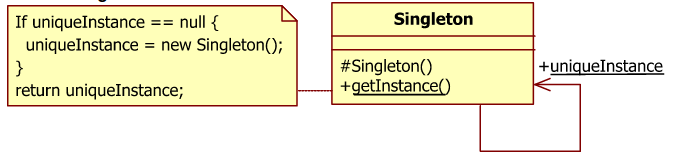
\includegraphics[scale=0.7]{img/singleton.png}
\end{figure}

Ce patron s'implémente assez facilement en créant un pointeur static dans la classe et
une méthode permettant de créer l'instance si elle ne l'a pas déjà été et de renvoyer
celle-ci. Exemple avec la classe \emph{World} :
\begin{figure}[!h]
  \centering
  \caption{Initialisation et méthode du singleton pour \emph{World}}
  \begin{lstlisting}[language=c++]
World* World::instance = nullptr;

World& World::getInstance()
{
    if (instance == nullptr)
        instance = new World();
    return *instance;
}
\end{lstlisting}
\end{figure}

On a copié la même chose pour la classe \emph{System}, cette duplication de code pourrait
être supprimée en faisant un \emph{template} c++ pour généraliser le singleton.

\subsubsection{Builder}
Le dernier patron de conception utilisé est un \emph{Builder} un peu détourné. Ici notre builder est l'entité \emph{Base} qui
a la possibilité de créer des \emph{Harvester} dans son environnement si il possède assez de ressources.

\begin{figure}[!h]
  \centering
  \caption{Diagramme de classe du patron \emph{Builder} (source: \href{http://www.goprod.bouhours.net/?page=pattern&pat_id=4}{Site de M.Bouhours})}
  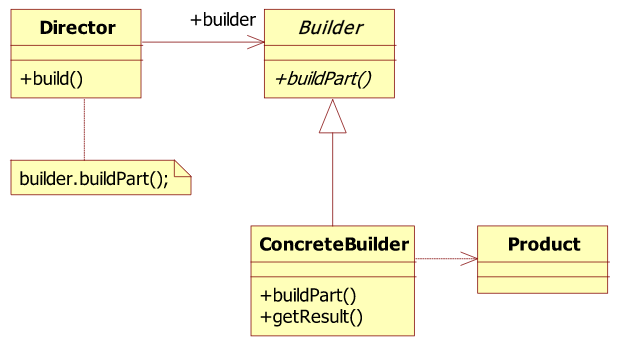
\includegraphics[scale=0.6]{img/builder.png}
\end{figure}

Ainsi, lorsqu'un \emph{Harvester} apporte une ressource à sa base et que celle-ci a assez de ressource nécessaire, il lui "ordonne" de
créer un autre \emph{Harvester} dans son environnement. L'implémentation de la méthode de création d'un \emph{Harvester} par une base
a été faite de la manière suivante :
\begin{figure}[!h]
  \centering
  \caption{Méthode de la classe \emph{Base} qui génère des \emph{Harvester}}
  \lstinputlisting[language=c++, firstline=37, lastline=49]{../Code/src/Entities/Base.cpp}
\end{figure}


% =========================================================== %
%                        Implémentation
% =========================================================== %

\newpage
\section{Implémentation}
\subsection{Les agents}
\subsubsection{Harvester}
On rappelle qu'un agent \emph{Harvester} (récolteur) à un rôle simple. Il parcourt aléatoirement le monde et lorsqu'il trouve une ressource
il la prend et la rapporte à la \emph{Base} à laquelle il est lié. Pour l'implémentation de cet agent, on a donc fait
en sorte qu'il possède un "état", qui décide de son comportement et a deux possibilités :
\begin{itemize}
  \item SEARCH, lorsque l'agent recherche une ressource et se déplace donc aléatoirement
  \item BRING, lorsqu'il possède une ressource et veut la ramener à sa base
\end{itemize}
\begin{figure}[!h]
  \centering
  \caption{Méthode \emph{move} et \emph{update} de la classe \emph{Harvester}}
  \lstinputlisting[language=c++, firstline=24, lastline=73]{../Code/src/Entities/Agent/Harvester.cpp}
\end{figure}
\vspace{8pt}
Ainsi la méthode commune aux différents agents (\emph{update}) pour le \emph{Harvester} n'est en fait que les conditions
pour passer d'un état à l'autre, plus le mouvement dans l'environnement. On a différencier ce dernier dans une méthode à part.
Ce mouvement dépend lui aussi de l'état du \emph{Harvester}. Si il est dans l'état \emph{SEARCH}, il cherche aléatoirement une case vide
dans son environnement de Moore d'ordre 1 et s'y déplace. Si il est dans l'état \emph{BRING}, il se déplace au plus court vers sa base.

\subsubsection{Hunter}
Le \emph{Hunter} se déplace aléatoirement dans un voisinage de Moore d'ordre 2 si il ne "voit" pas d'agent \emph{Harvester} dans un
voisinage de Moore d'ordre 3. Si il voit un \emph{Harvester} et qu'il est à moins de 2 cases, il se déplace sur sa position et le
mange, sinon il se déplace au plus proche vers lui.
\begin{figure}[!h]
  \centering
  \caption{Méthode \emph{update}  de la classe \emph{Hunter} : interactions avec les \emph{Harvester}}
  \lstinputlisting[language=c++, firstline=26, lastline=67]{../Code/src/Entities/Agent/Hunter.cpp}
\end{figure}

De plus, le \emph{Hunter} à une "vie", qui diminue lorsqu'il ne mange pas et
augmente lorsqu'il mange. Plus exactement cette vie est composée de 3 "stades" :
\begin{itemize}
  \item vert, si il ne mange pas pendant 5 étapes, il passe au orange. Si il mange il créer un autre \emph{Hunter}
  \item orange, si il ne mange pas pendant 5 étapes, il passe au rouge. Si il mange il passe au vert
  \item rouge, si il ne mange pas pendant 5 étapes, il meurt. Si il mange il passe au orange
\end{itemize}
\begin{figure}[!h]
  \centering
  \caption{Méthode \emph{update}  de la classe \emph{Hunter} : gestion de sa vie}
  \lstinputlisting[language=c++, firstline=69, lastline=115]{../Code/src/Entities/Agent/Hunter.cpp}
\end{figure}
Pour cette gestion de vie, il aurait été intéressant de créer une interface permettant de gérer les durées de chaque stade (vert, orange
et rouge) pour observer les changements de comportement.


\newpage
\subsection{World}
C'est l'objet \emph{World} qui permet à ces deux types d'agents d'interagir avec leur environnement. On remarque dans les implémentations
précedentes plusieurs appels à des méthodes de la classe \emph{World} :
\begin{itemize}
  \item getEnvironnement, qui permet d'obtenir l'ensemble des cases (sous forme d'un tableau) autour d'un point donné dans un voisinage de Moore dont on précise l'ordre
  \begin{figure}[!h]
    \centering
    \caption{Méthode \emph{getEnvironnement}  de la classe \emph{World}}
    \lstinputlisting[language=c++, firstline=97, lastline=110]{../Code/src/Utils/World.cpp}
  \end{figure}

  \item findRandomPositionInEnvironnement, qui prend un "environnement" en paramètre et cherche un type d'entité ou les cases vides. Si il
  y en a plusieurs, elle choisit aléatoirement entre. Cette méthode renvoie la position de l'entité ou de la case vide trouvée.
  \begin{figure}[!h]
    \centering
    \caption{Méthode \emph{findRandomPositionInEnvironnement}  de la classe \emph{World}}
    \lstinputlisting[language=c++, firstline=68, lastline=95]{../Code/src/Utils/World.cpp}
  \end{figure}
\end{itemize}

Pour utiliser l'aléatoire, l'objet \emph{World} a une instance d'un générateur Mersenne Twister et utilise \emph{std::shuffle} fournis par la STL du c++.

Le monde dans lequel évoluent les agents est un "tore". C'est-à-dire que le haut est relié au bas et la gauche est reliée à la droite.
Afin de faire cela, on a doté la classe \emph{World} d'accesseurs particuliers. En effet, pour accèder à un point du monde, on passe
en paramètre un \emph{Point} qui, si il dépasse les coordonnées du monde, est ramené aux coordonnées correspondantes en supposant que le
monde est un tore. Par exemple, si le monde fait 20 de haut et 20 de large, les coordonnées (4, 3) représentent la même case que les
coordonnées (24, 3) ou (4, 43) ou (44, 63).
\begin{figure}[!h]
  \centering
  \caption{Représentation 3D d'un \emph{Tore}}
  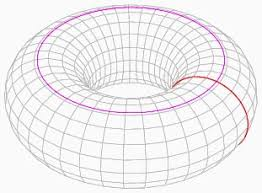
\includegraphics[scale=1]{img/tore.jpeg}
\end{figure}
\begin{figure}[!h]
  \centering
  \caption{Méthode pour accèder à une case du monde de la classe \emph{World}}
  \lstinputlisting[language=c++, firstline=129, lastline=135]{../Code/src/Utils/World.cpp}
\end{figure}

\subsection{System}
Depuis que l'on a séparé les fonctionnalités en deux classes, \emph{System} et \emph{World}, la classe \emph{System} est très simple.
Elle ne fait qu'ajouter et supprimer des agents d'un tableau et de mettre à jour tous les agents vivants
dans ce tableau.
Ainsi, avant les "updates" des agents, on mélange l'ordre pour que le sens d'appel ne soit jamais le même. On utilise pour cela le générateur
aléatoire Mersenne Twister de \emph{World}.

Pour la suppression des agents qui "meurent" à cette étape, on ne peut pas le faire dans la boucle qui appelle les "updates" puisqu'on
modifierait la taille du tableau qu'on parcourt. La solution est que les agents ne se "suppriment" pas mais indiquent qu'ils sont morts
grâce à la méthode \emph{isDead}. Une fois la boucle d'updates finie, on utilise le \href{https://en.wikipedia.org/wiki/Erase%E2%80%93remove_idiom}{Erase-Remove Idiom}
pour retirer tous les agents morts du tableau.

Pour l'ajout d'agents (via les \emph{Hunter} lorsqu'ils mangent ou via les \emph{Base} lorsqu'elles on assez de ressources), le principe
est le même : on ne peut pas modifier les tableau lorsqu'on le parcourt. On a donc un \emph{buffer} qui contient tous les agents qu'on
désire ajouter et lorsqu'on a fini les updates, on ajoute tous le contenu du buffer dans le tableau principal.

\newpage
\begin{figure}[!h]
  \centering
  \caption{Méthodes d'ajout et \emph{update} de la classe \emph{System}}
  \lstinputlisting[language=c++, firstline=35, lastline=71]{../Code/src/System.cpp}
\end{figure}

\newpage
\section{Analyse de performances}
Nous avons décidé d'étudier l'impact des options d'optimisations de g++ sur la rapidité d'exécution de notre simulation multi agents.
Pour celà nous avons compilé le programme avec l'option -O0 et avec l'option -O3, en renommant à chaque fois le nom de l'exécutable. Nous avons ensuite exécuté le programme en passant par l'outil perf.
\begin{mdframed}[backgroundcolor=light-gray, roundcorner=20pt,
  innerleftmargin=20, innertopmargin=1, innerbottommargin=1, 
  outerlinewidth=1, linecolor=darkgray]
  \begin{lstlisting}[language=Bash]
perf stat ./bin/sma_O0 --log-file
perf stat ./bin/sma_O3 --log-file\end{lstlisting}
\end{mdframed}
Il a été choisi de lancer la simulation avec une sortie sur un fichier.
Nous avons également modifié les paramètres initiaux de la simulation pour qu'elle s'exécute pendant un temps assez long, quelques secondes. Cela permettant sûrement de refléter un peu plus un changement sur les performances, même minim.
\subsection{Mesures}
L'ensemble des mesures effectuées sont disponnibles dans un fichier, ouvrable avec le programme libre office. Voici tout de même un graphique résumant les valeurs mesurées.
\begin{figure}[!h]
  \centering
  \caption{Temps d'exécution de la simulation selon différentes options de compilation}
  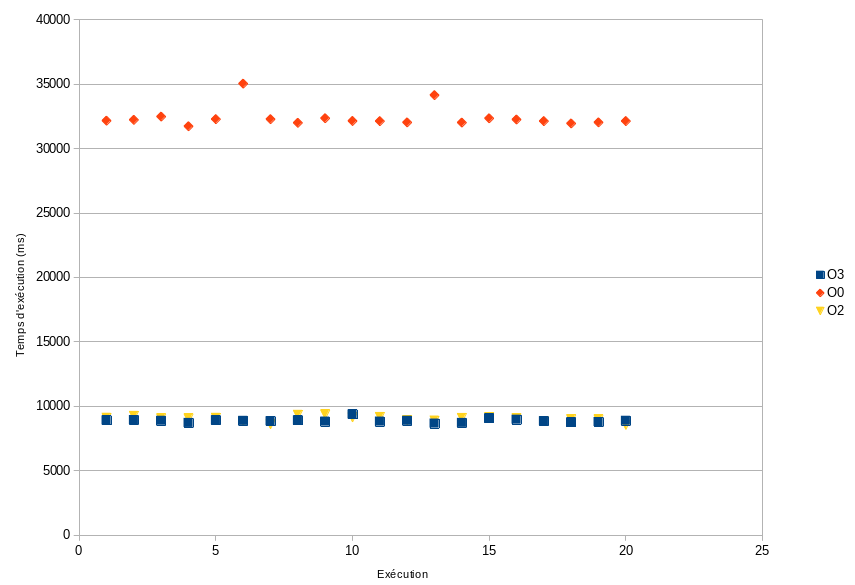
\includegraphics[width=\textwidth]{img/exec_plot.png}
\end{figure}
\subsection{Interprétation des résultats}
On remarque très nettement une différence entre une compilation sans optimisations (-O0) et une compilation avec (-O2 et -O3).
Nous ne nous attendions pas à une différence si marquée. Cependant la différence entre les deux dernières options est très faible.
Le calcul de leur intervalle de confiance, nous indique même qu'ils n'y a statistiquement aucune différence. En effet, ils se chevauchent.
Les valeurs exactes sont également dans le document joint.

Il est intéressant de noté que chaque exécution donne le même résultat, même si les options de compilation ne sont pas les mêmes.

On peut aussi relevé que le fait d'avoir une sortie à notre programme impose un ralentissement. Une utilisation de la simulation comme une boite noir ne donnant que le résultat final, aurait certainement permi de bien meilleure performance. L'impact des options d'optimisation aurait certainement était d'autant plus notable, et les temps d'exécution plus proche de la moyenne.

\newpage
\appendix
\section{Manuel d'utilisation}
Un fois compilé (\emph{make -j}), on execute le programme avec la commande :
\begin{lstlisting}
  $ bin/sma --<option>
\end{lstlisting}
Où les options possibles pour executer le programme sont :
\begin{itemize}
  \item draw permet d'avoir un visuel plus fluide
  \item log permet d'avoir chaque étape écrite dans le terminal (equivalent à sans options)
  \item log-file permet d'avoir la sortie du programme dans un fichier "output.log"
  \item log-draw permet de combiner --draw et --log-file
\end{itemize}

\section{Compilation}
Un makefile a été utilisé pour simplifier la compilation de ce TP. Voici son contenu
\lstinputlisting[language=c++, firstline=1, lastline=57]{../Code/makefile}

On a seulement besoin de la STL du c++. Notamment de la bibliothèque \href{https://en.cppreference.com/w/cpp/numeric/random}{\emph{<random>}}
pour générer tous les nombre pseudo-aléatoires du programme, de la bibliothèque \href{https://en.cppreference.com/w/cpp/container/vector}{\emph{<vector>}}
et de \href{https://en.cppreference.com/w/cpp/algorithm}{\emph{<algorithm>}} afin de gérer les agents et les entités dans le système et le monde.

\section{Documentation}
\changeurlcolor{blue}\href{run:../Documentation/latex/refman.pdf}{Lien vers la documentation Doxygen}

\end{document}